% ============================ 一、问题定义与科学价值 ============================
\section{问题定义与科学价值}
\label{sec:problem}

\subsection{项目名称与参赛方向}

\textbf{虚拟细胞：面向酿酒酵母扰动蛋白质组的机制受限预测系统与可质询的探索环境}（代号 \code{VC-Yeast}）。参赛方向：赛道三「前沿探索 · AI for Research」\textbf{算法赛题一：虚拟细胞}，统一开放榜。

主榜任务为：从组委会提供的 \code{train\_val} 数据中学习跨\textbf{菌株、化学扰动、培养基、温度、时间点与测量上下文}的蛋白质组响应规律，对测试集预测完整的 log$_2$ 蛋白丰度向量。本方案同时在一个方法学问题上给出可复核的实证回答：\emph{引入外部生物学知识，是否真的带来预测增益}。

\subsection{独立复算的数据规格：与修订后手册逐项一致}
\label{sec:spec}

我们在阶段 1 的质控中\textbf{独立测得}数据规格，此处与修订后手册的表述逐项对照——这既是对手册的核对，也是对我们读数管线的交叉检验：

\begin{table}[H]
\centering\small
\caption{\textbf{数据规格的独立复算与手册对照。} 左列为修订后手册（2.2 节第 9--11 条）的表述，右列为我们在 \file{evidence/metadata\_profile.json} 与 \file{evidence/qc\_summary.json} 中独立测得的值。全部一致。}
\label{tab:spec}
\begin{tabular}{llll}
\toprule
项目 & 手册表述 & 我方独立复算 & 判定 \\
\midrule
\code{train\_val} 样本量 & 8\,958 & 8\,958（去重后 8\,958，重复 0） & 一致 \\
\code{test} 样本量 & 4\,454 & 4\,454（与 \code{train\_val} 交集 0） & 一致 \\
蛋白维度 & 5\,243 & 5\,243（朴素逗号切分会误得 5\,245，见表 \ref{tab:defects}） & 一致 \\
菌株数 & 6 & 6（\code{train\_val} 5 个 $+$ 仅测试集出现的 \textbf{CRD}） & 一致 \\
化合物数 & 56 & 57 个扰动标签 $-$ 1 个质控标签 $=$ \textbf{56} & 一致 \\
质控样本 & \code{pert\_id = 48} 单列 & \code{Quality Control} 共 118 例，\textbf{不参与化学扰动预测} & 一致 \\
培养基 / 温度 / 时间点 & 2 / 2 / 6 & 2 / 2 / 6（各因子间并非完全交叉） & 一致 \\
\bottomrule
\end{tabular}
\end{table}

一个细节值得写出来：\code{pert\_id} \emph{不是}化合物身份——15 个 \code{pert\_id} 映射到多个化合物（\code{\#2} 在一个批次是 DMSO、在另一批次是 EDTA）。我们因此改用 \code{perturbation\_no\_concentration} 作为实体键。若沿用 \code{pert\_id} 匹配溶剂对照，会把不同批次的两种试剂混为一谈，而这类错误\textbf{不会抛出任何异常}。

\subsection{科学问题与当前争议}

「AI 虚拟细胞」被明确表述为一个可操作的研究纲领：构建能在计算中预测细胞对未见扰动之响应的模型，把实验搜索空间从穷举转向定向\citep{Bunne2024VirtualCell}。其前身是单细胞扰动图谱的规模化\citep{Dixit2016PerturbSeq,Replogle2022GenomeScale,Norman2019GIManifolds}与随之建立的公开基准\citep{Rood2024PerturbationAtlas,Roohani2025VirtualCellChallenge,Luecken2025OpenProblems}；方法侧则形成了条件生成模型\citep{Lotfollahi2019scGen,Lotfollahi2023CPA,Hetzel2022chemCPA}、图先验驱动预测\citep{Roohani2024GEARS}与单细胞基础模型\citep{Cui2024scGPT,Theodoris2023Geneformer,Adduri2025State}的谱系。

但这一谱系近期遭遇严肃反诘：多项独立评估指出，在若干标准设定下线性基线甚至「训练集均值」基线即可与复杂深度模型持平乃至更优\citep{AhlmannEltze2025LinearBaselines,Kernfeld2025ExpressionForecasting,Csendes2025BenchmarkingFoundation,Wei2026scPerturBench}。其实质并非「深度模型无用」，而是\textbf{评测设计决定了什么算作进步}。本赛题的价值恰在于把这一点写进规则——S1（新化合物）、S2（新菌株）、S3（双新）强制模型在\emph{实体层面}外推，而非在样本层面插值。

\textbf{统一开放榜把这一点推到了逻辑终点。} 修订说明的论证是：外推天然需要引入外部信息，不引入实体表征，模型面对未见实体时只能将其当作空白类别处理。我们完全同意，并愿意补充一句更锋利的话：\emph{一个把未见实体当作空白类别的模型，其在 S1/S2 上的分数只能来自协变量结构与群体均值，而不可能来自实体本身}——这正是我们在 \S\ref{sec:s1confound} 中定量证实的现象。

读出层为\textbf{蛋白质组}而非转录组，是一个实质性选择：酵母中蛋白与 mRNA 丰度的相关性长期被测定为中等水平\citep{Gygi1999Correlation}，偏差主要来自翻译效率与蛋白周转\citep{Vogel2012Insights,Liu2016Dependency}，因而从转录预测蛋白无法替代直接的蛋白层建模。酵母则提供了此类建模所需的全部支撑：完整基因组\citep{Goffeau1996Life6000,engel2022sgd}、全基因组缺失突变体库\citep{Giaever2002DeletionCollection}、化学基因组学谱\citep{Hillenmeyer2008ChemicalGenomics}、全局遗传互作网络\citep{Costanzo2016GlobalGI}、胁迫响应程序\citep{Gasch2000ESR}与调控网络扰动图谱\citep{Kemmeren2014RegulatoryNetworks}，以及蛋白层的绝对定量与大规模扰动图谱\citep{Lahtvee2017AbsoluteQuant,Ho2018ProteomeUnification,Messner2023ProteomicLandscape}。菌株层面另有 1\,011 个 \Sc{} 分离株的群体基因组资源\citep{peter2018_1011genomes}——它正是修订说明推荐的菌株表征来源，也正是我们当前的短板所在。

\subsection{任务形式化}

记样本 $i$ 的设计条件 $c_i=(\text{菌株},\text{化合物},\text{培养基},\text{温度},\text{时间})$、测量上下文 $x_i=(\text{数据源},\text{仪器},\text{培养板},\text{蛋白孔})$，目标为 $\bm{y}_i\in(\mathbb{R}\cup\{\mathrm{NaN}\})^{5243}$，模型给出 $\hat{\bm{y}}_i=f(c_i,x_i)$。评分同时作用于绝对丰度与倍数变化
\begin{equation}
\bm{\Delta}_i=\bm{y}_i-\operatorname{median}\{\bm{y}_j:j\in\mathcal{C}(i)\},
\label{eq:delta}
\end{equation}
其中 $\mathcal{C}(i)$ 为按\textbf{冻结规则}匹配的溶剂对照集合。真值与预测两侧使用\emph{同一个}冻结锚点，故锚点不参与相关性竞争。S1/S2 模块进一步在减去冻结群体均值后计算残差相关：
\begin{equation}
\text{S1}:\operatorname{PCC}(\bm{\Delta}_{\text{pred}}-\bm{\mu}_{\text{ctx}},\,\bm{\Delta}_{\text{true}}-\bm{\mu}_{\text{ctx}}),\qquad
\text{S2}:\operatorname{PCC}(\bm{\Delta}_{\text{pred}}-\bm{\mu}_{\text{drug}},\,\bm{\Delta}_{\text{true}}-\bm{\mu}_{\text{drug}}).
\label{eq:resid}
\end{equation}
两侧减去同一个 $\bm{\mu}$，使一个只复现群体均值的模型残差方差为零、相关系数无定义并按下限记 0——这是评分设计对平凡解的惩罚机制。修订说明明确「未见」指该实体\emph{不在训练划分中}，与参赛队能否看到其真值无关；我们的划分审计正是按此定义实现（\S\ref{sec:protocol}）。

\subsection{数据本身提出的三个技术性科学问题}

\begin{figure}[H]
\centering
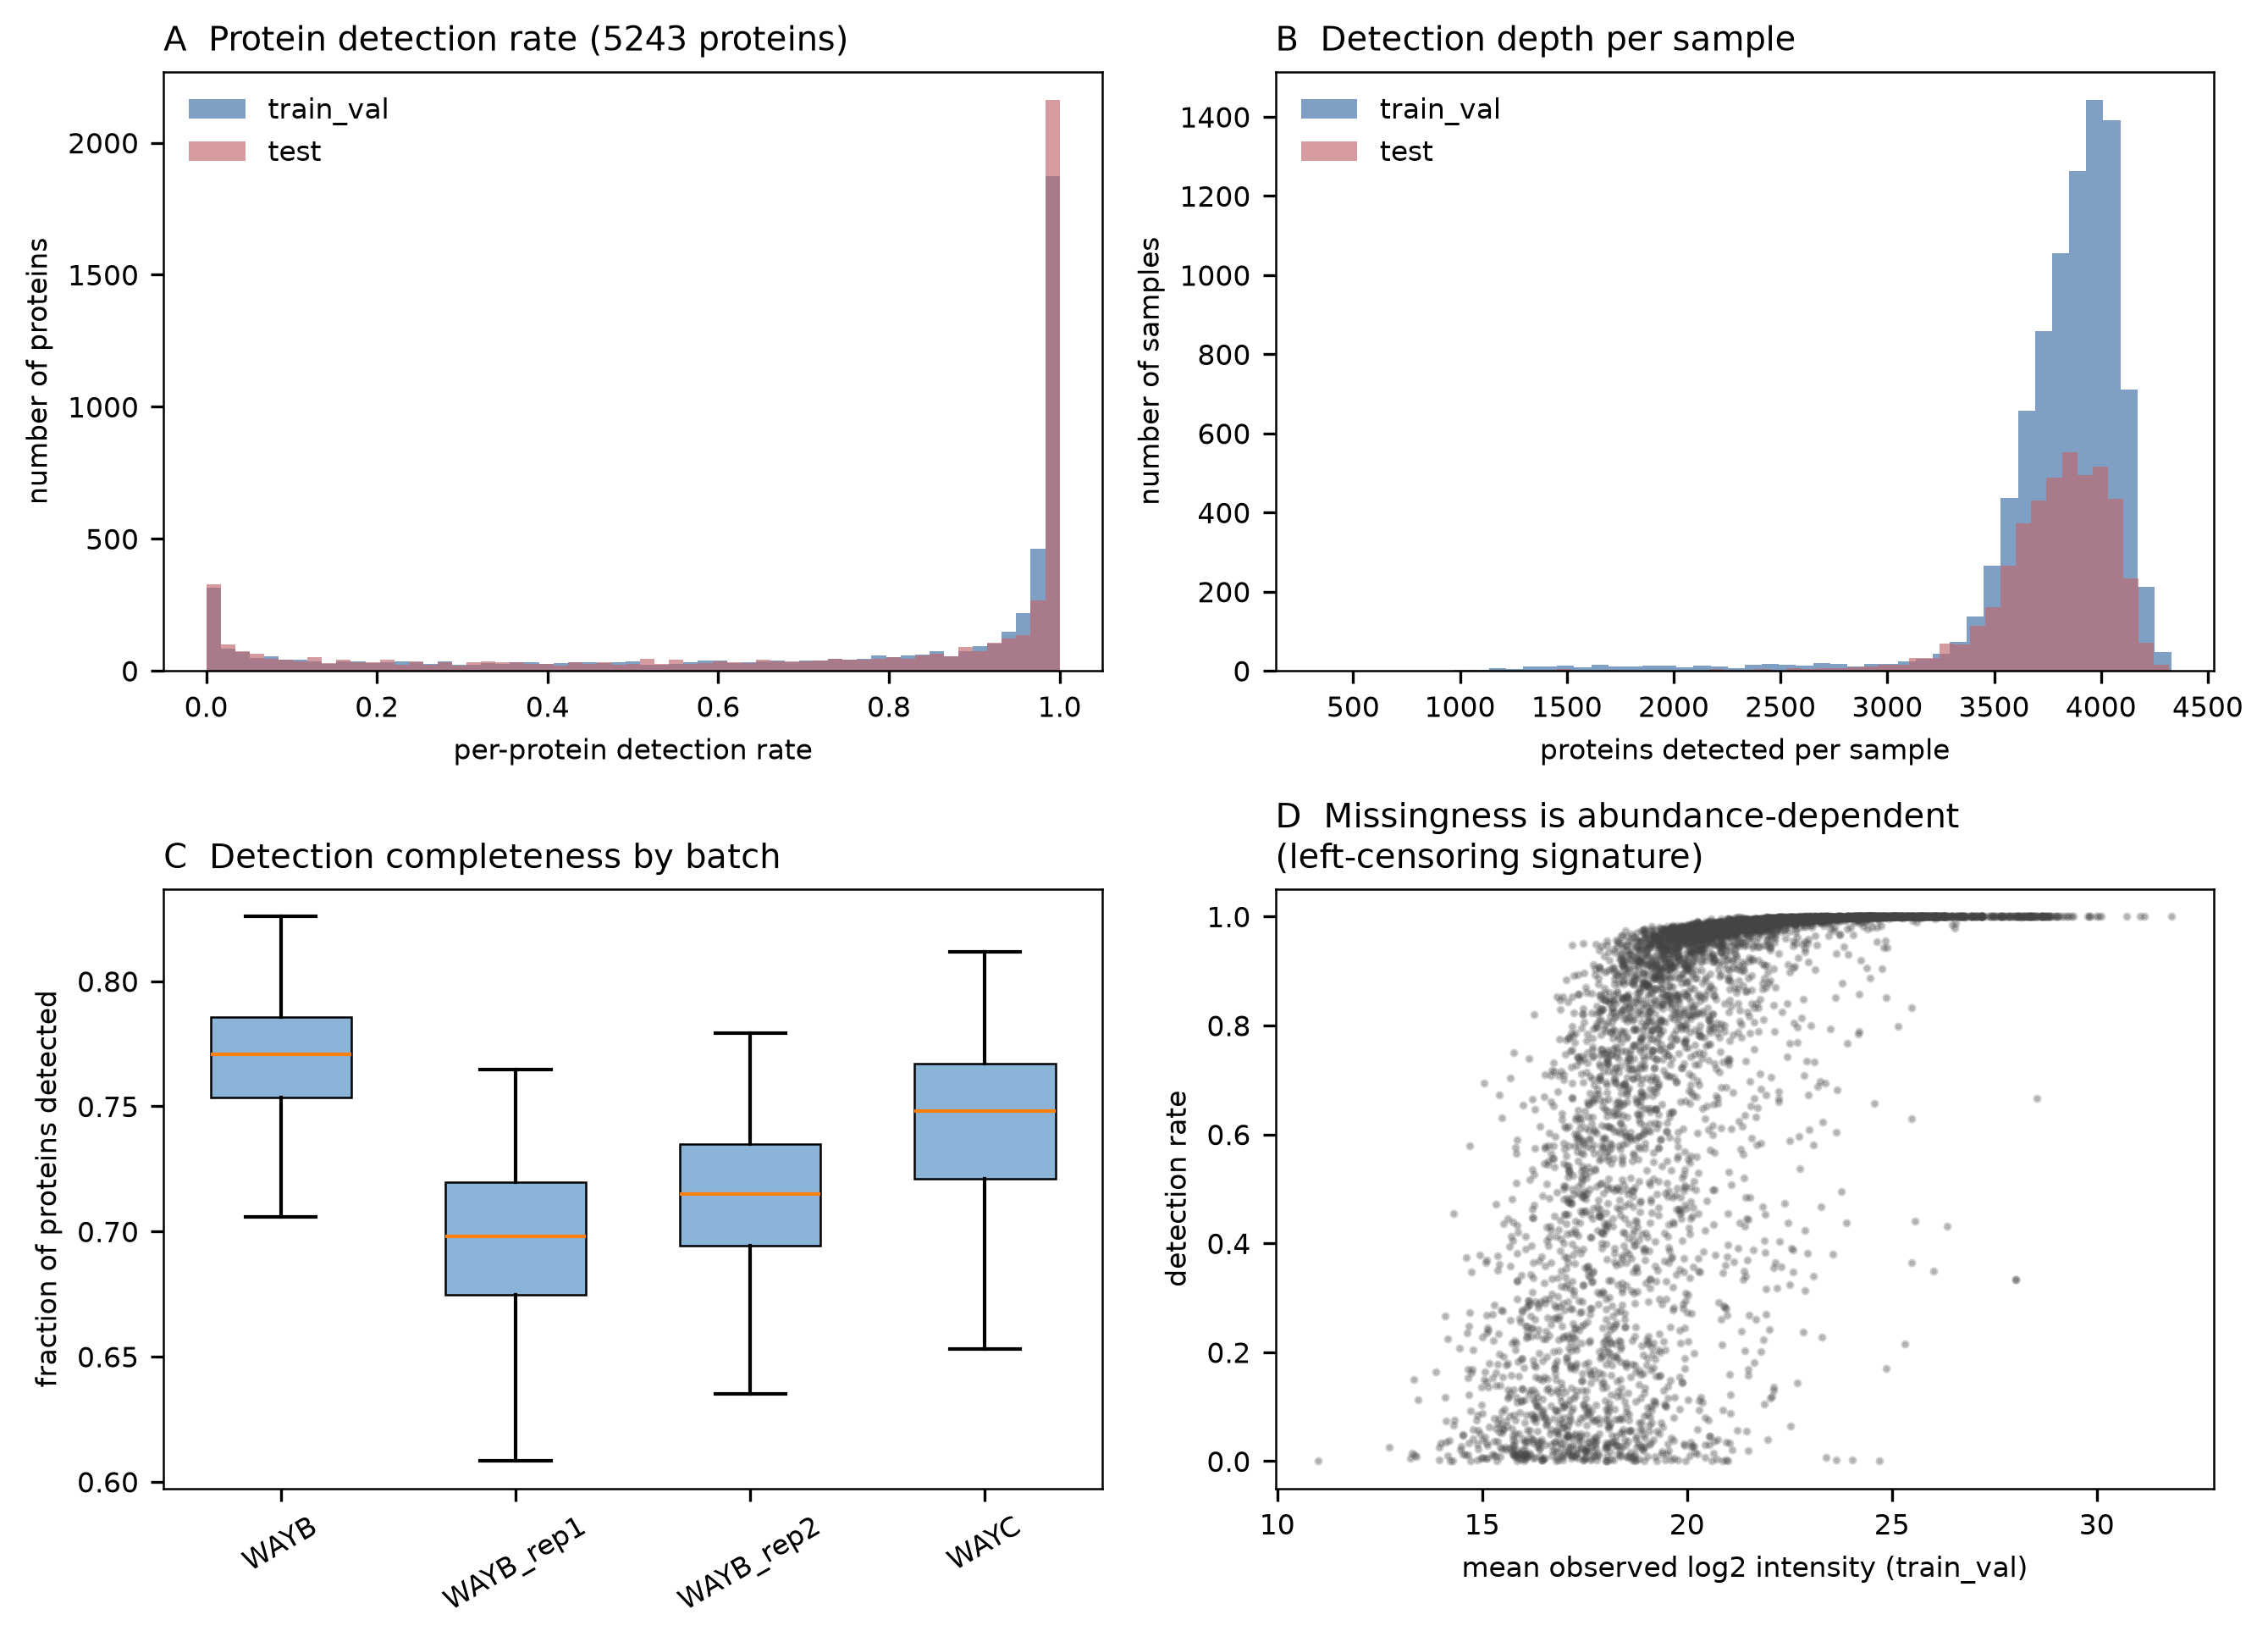
\includegraphics[width=0.93\textwidth]{figures/eda_missing_values.png}
\caption{\textbf{缺失结构与左删失的直接证据。}
\textbf{A} 逐蛋白检出率分布在 0 与 1 两端双峰（\code{train\_val} 中 186 个蛋白从未检出、263 个蛋白全样本检出），训练验证与测试两侧形态一致；
\textbf{B} 逐样本检出深度分布（\code{train\_val} 中位 3\,891 个蛋白）；
\textbf{C} 按批次的检出完整度；
\textbf{D} \emph{缺失依赖丰度}——检出率与平均 log$_2$ 丰度的 Spearman $\rho=0.860$（$n=5\,057$ 个统计量有限的蛋白，本次由 \file{evidence/qc\_metrics\_proteins.csv} 重算）；按检出率五分位分组，观测 log$_2$ 丰度中位数从 17.53 单调升至 24.42。
这是数据依赖型缺失（MNAR）的教科书形态，而非随机缺失。原始数值为线性质谱强度，经 log$_2$ 变换与逐样本中位数中心化后重对齐到\textbf{仅由训练行计算}的参照偏移 21.3286；\textbf{全流程不做任何填补}。}
\label{fig:qc}
\end{figure}

\paragraph{问题一：缺失是测量过程的一部分，不是数据缺陷。}
\code{train\_val} 27.353\,\%、\code{test} 27.851\,\% 的单元为空，且两侧\textbf{精确零值计数均为 0}——缺失以空字段编码，从不与真实零混淆（图 \ref{fig:qc}）。这一形态在定量蛋白质组学中被反复刻画\citep{Lazar2016MissingNatures,Karpievitch2012NormImpute,WebbRobertson2015Imputation}，并且均值/中位数填补已知会系统性抬高低丰度估计\citep{Wei2018MissingValue,Kong2022MissingValues}。因此正确的建模对象不是「填补后的完整矩阵」，而是\textbf{「观测值 $+$ 删失指示」的联合}。

\paragraph{问题二：数据中最强的方差不是生物学。}
批次效应在组学中是长期问题\citep{Leek2010BatchEffects,Johnson2007ComBat,Cuklina2021BatchProteomics}，且在与生物学因素共线时其「校正」本身会引入偏倚\citep{Nygaard2016BatchLimits}。本赛题的特殊之处在于：\textbf{测量上下文是官方输入特征的一部分}，其设计意图正是让模型吸收测量过程引入的变异。这把批次从「要消除的噪声」变成「要正确使用的协变量」，同时带来一个隐患——式 \eqref{eq:resid} 中的 $\bm{\mu}_{\text{ctx}}$ 是\emph{批次盲}的，于是一个批次感知的条件均值可以在 S1 上不劳而获。我们在两个队列上都实测确认了这一隐患（\S\ref{sec:s1confound}）。

\begin{figure}[H]
\centering
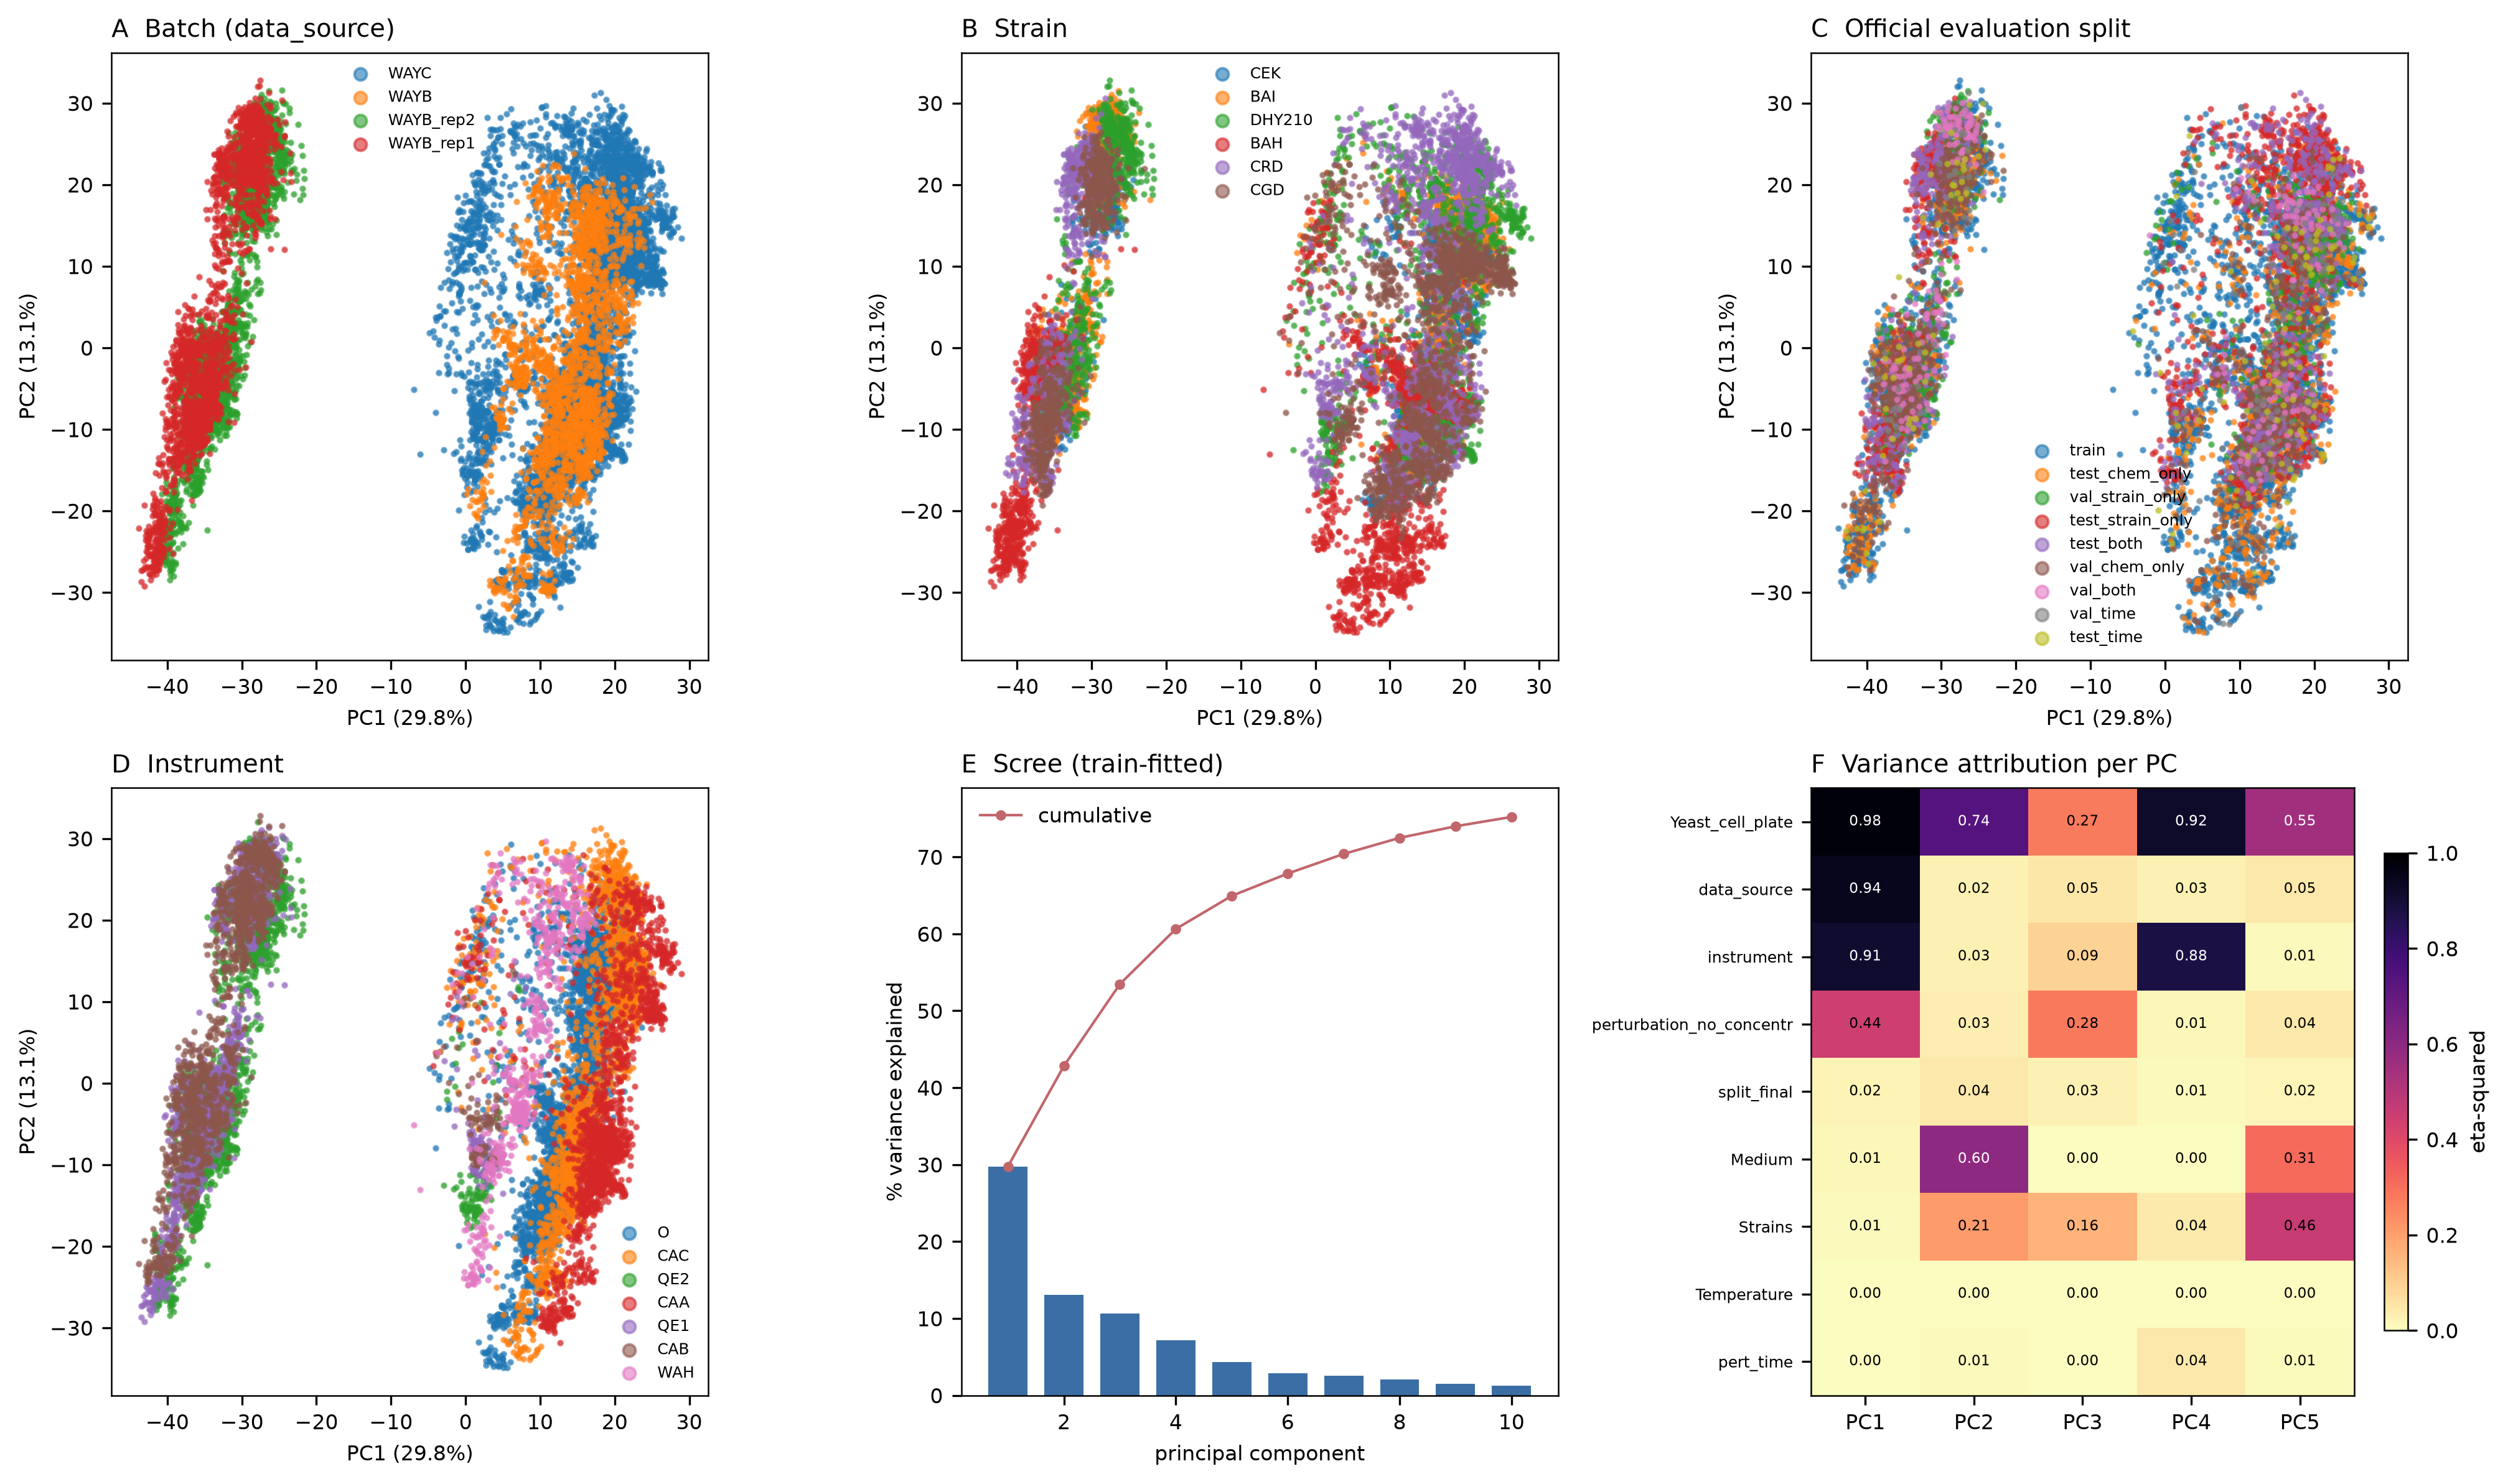
\includegraphics[width=0.95\textwidth]{figures/eda_pca_batch_effects.png}
\caption{\textbf{主成分结构与方差归因。} A--D 为 PC1--PC2 散点，分别按批次、菌株、划分与仪器着色；E 为训练集拟合的碎石图；F 为各因素对前若干主成分的 $\eta^2$ 方差归因热图。PC1（解释 29.766\,\% 方差）由培养板（$\eta^2=0.9774$）、数据源（0.9445）与仪器（0.9139）主导，\textbf{菌株仅 0.0093}、温度 0.0004、时间 0.0003；生物学信号首次出现在 PC2（培养基 0.5966、菌株 0.2090）与 PC5（菌株 0.4604）。PCA 仅在训练行上拟合，其余划分与测试集只做投影；另有一项填补敏感性检验显示前四主成分子空间在 1\,\% 分位填补下的平均重叠为 0.994。}
\label{fig:pca}
\end{figure}

\paragraph{问题三：药物机制在该设计下不可识别。}
训练划分可用的分子化合物仅 37 种（40 个化学标签减去 Water、DMSO 与质控），蛋白列 5\,243 个。$37\times5\,243$ 个待估接合单元只有 37 个独立的化合物级对比支撑。这不是估计效率问题，而是设计的秩亏问题。直接推论是：\textbf{机制必须从数据集之外导入，并用与训练无关的证据独立验证}\citep{gaulton2017chembl,zdrazil2024chembl}——统一开放榜的规则调整，正是承认了这一点。

\subsection{科学价值}

\begin{figure}[H]
\centering
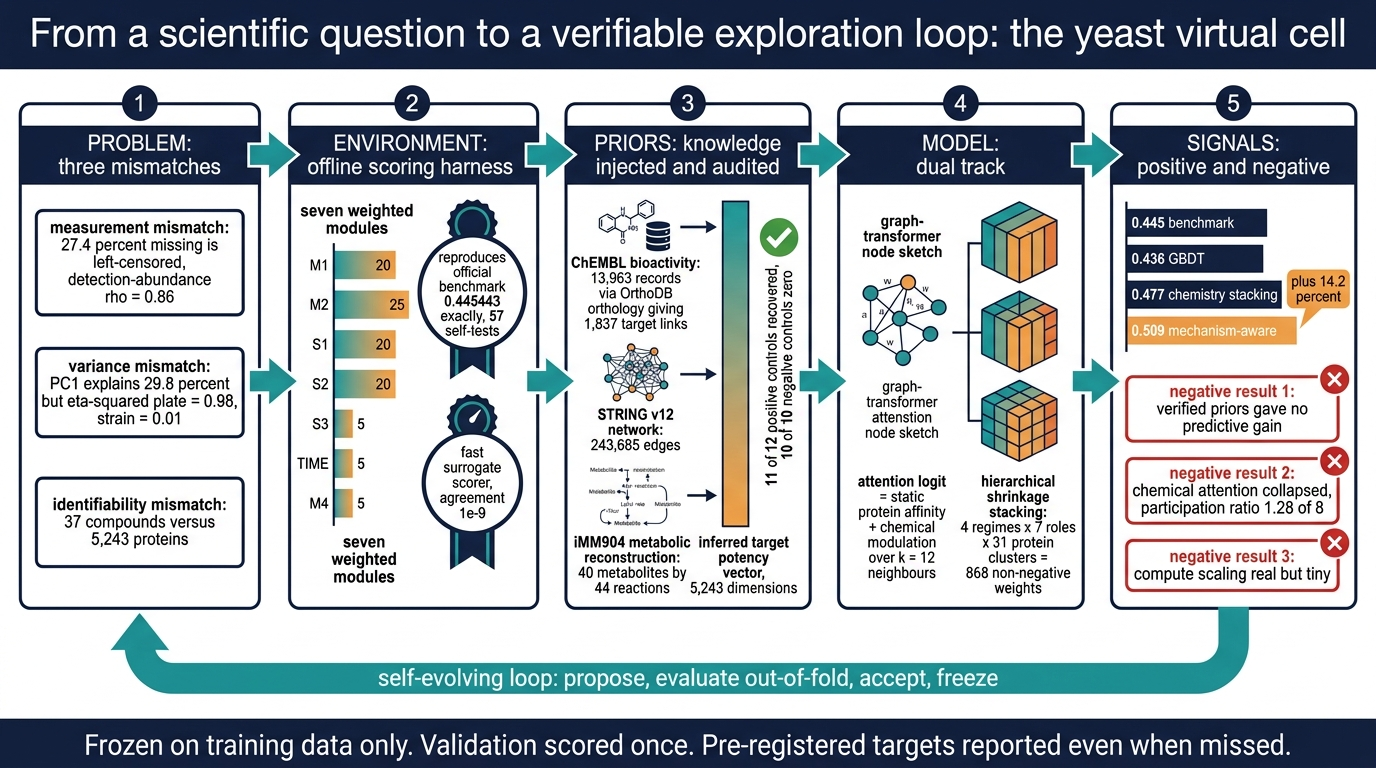
\includegraphics[width=\textwidth]{figures/ga_submission2.png}
\caption{\textbf{探索闭环总览：从科学问题到可验证的循环。} 五个环节依次为问题（三重错配）、环境（离线七模块 harness 与快速代理评分器）、先验（三源知识汇聚为靶点效力向量并经药理学正负对照验证）、模型（双轨结构）、信号（正向成绩与三项负结果并列）；底部回环为自演化环路，底栏为三条纪律。此图与图 \ref{fig:ga} 互补：图 \ref{fig:ga} 给出\emph{系统构成}，本图给出\emph{工作流闭环}。}
\label{fig:loop}
\end{figure}

\textbf{对虚拟细胞纲领。} 当前争议的焦点是评测：模型究竟学到了扰动生物学，还是条件均值\citep{AhlmannEltze2025LinearBaselines,Csendes2025BenchmarkingFoundation}。本方案提供三项可直接迁移的贡献。其一，\textbf{给出零假设的正确位置}：残差相关的空值下限并非 0，而是（验证队列，残差 PCC 子度量）0.237（新化合物）、0.179（新菌株）、0.221（双新）、0.108（时间）——一个把 $\Delta$ 预测为全零的平凡模型即可取得，因此任何改进都必须以此为参照；\NEW{}我们在测试队列上重算了同一组下限（表 \ref{tab:rubric}），二者同量级但不同数值，说明\emph{下限本身是队列依赖的}，跨队列比较分数时必须同时报告下限。其二，\textbf{证明评分口径本身可被平凡解利用}：批次盲的残差基线让批次条件均值在 S1 上免费得分，且这一诊断在两个队列上同向复现，因此它对任何采用「减去群体均值再算相关」口径的基准都构成警示。其三，\textbf{把知识注入从叙事变成可证伪实验}：一个通过全部药理学对照的先验，仍可能在预测上完全无效——这两件事必须分别报告。

\textbf{对蛋白质组学与酵母生物学。} 方法上，我们主张把检出限作为\emph{似然}的一部分（\S\ref{sec:tobit}），使模型在低丰度区间输出「低于检出限的概率」而非一个被填补规则决定的数值；这对任何以 DIA/DDA 定量为输入的预测任务直接可用\citep{Gillet2012SWATH,Demichev2020DIANN,Choi2014MSstats,Ritchie2015Limma}。资源上，我们产出的\textbf{推断靶点效力向量}把 ChEMBL 中 1\,921 个靶点上的 13\,963 条结合亲和记录经 OrthoDB 直系同源关系\citep{kuznetsov2023orthodb}投射到 5\,243 个被测酵母蛋白的\emph{同一坐标轴}上，可直接作为其他酵母化学基因组学分析的先验。

\textbf{对 AI for Research 方法论。} 我们认为最容易被跳过、也最关键的一环，是\textbf{让系统能够发现并报告自己的错误}。本项目工程体系捕获的 20 项缺陷中，若干项若未被捕获将直接导致错误结论：按 \code{pert\_id} 匹配对照会把不同批次的 DMSO 与 EDTA 混为一谈；盐析处理会把顺铂静默还原为氨（分子量 17.03 对 300.05）；一个过严的动态范围门控中止了阶段 5 的导出，而这个门控正是本系统自己在阶段 4 引入的。最后一例尤其重要——\textbf{检查装置本身不能自证}。与此相关，近期 AI 科研智能体工作\citep{boiko2023coscientist,lu2024aiscientist,gottweis2026coscientist,swanson2025virtuallab}普遍强调「自主发现」而较少讨论「自主证伪」；本方案把后者作为红线写进协议。
